% Documento standalone: Reporte de Benchmark LwM2M
% Genera: benchmark_report.pdf
\documentclass[11pt,spanish,letterpaper]{article}

\usepackage[utf8]{inputenc}
\usepackage[spanish,es-tabla]{babel}
\usepackage{amsmath,amssymb}
\usepackage{graphicx}
\DeclareGraphicsExtensions{.png,.pdf,.jpg,.jpeg}
\usepackage{float}
\usepackage{booktabs}
\usepackage{tabularx}
\usepackage{longtable}
\usepackage{subfigure}
\usepackage{array}
\usepackage[rgb,table]{xcolor}
\usepackage[hidelinks]{hyperref}
\usepackage[margin=2.5cm]{geometry}
\usepackage{fancyhdr}

\pagestyle{fancy}
\fancyhf{}
\fancyhead[L]{\small Benchmark LwM2M --- Datos Experimentales}
\fancyhead[R]{\small J.S. Giraldo --- Tesis M.Sc. 2026}
\fancyfoot[C]{\thepage}

\title{\textbf{Benchmark LwM2M del Firmware Final v0.15.1}\\[0.5em]
\large Datos experimentales del nodo IoT real\\
ami-esp32c6-2434 + Emsitech P2000-T}
\author{Juan Sebastián Giraldo\\
\small Maestría en Ingeniería --- Universidad Nacional de Colombia}
\date{Marzo 2026}

\begin{document}

\maketitle
\thispagestyle{fancy}

% ============================================================
\section{Descripción del Caso de Estudio}
% ============================================================

Se presenta el benchmark completo del nodo IoT real \textbf{ami-esp32c6-2434}
(XIAO ESP32-C6, Zephyr RTOS) conectado vía Thread/LwM2M al servidor Leshan,
midiendo un contador inteligente \textbf{Emsitech P2000-T} mediante protocolo
DLMS/COSEM sobre RS-485.

El benchmark evalúa el \textbf{firmware final v0.15.1} en 4 escenarios de
intervalo CoAP Observe (baseline, 1\,s, 5\,s, 10\,s), midiendo:
\begin{itemize}
    \item Completitud de \emph{keys} LwM2M reportadas (de 16 posibles)
    \item \emph{Throughput} (mensajes/segundo)
    \item Intervalo entre llegadas (IAT) por recurso
    \item Calidad de señal Thread (RSSI, LQI)
    \item Utilización del canal 802.15.4 y sobrecarga de protocolos
\end{itemize}

% ============================================================
\section{Análisis del Firmware Final v0.15.1}
% ============================================================

La Tabla~\ref{tab:v0151-detail} resume el rendimiento de v0.15.1 por
escenario Observe.

\begin{table}[htbp]
\centering
\caption{Detalle de rendimiento v0.15.1 por escenario Observe}
\label{tab:v0151-detail}
\begin{tabular}{lcccc}
\toprule
\textbf{Métrica} & \textbf{Baseline} & \textbf{1\,s} & \textbf{5\,s} & \textbf{10\,s} \\
\midrule
Mensajes totales     & 47    & 119   & 29    & 0 \\
Throughput (msgs/s)  & 0,261 & 0,661 & 0,161 & 0,000 \\
Keys reportadas (/16)& 16    & 16    & 16    & 0 \\
Duración captura (s) & 180   & 180   & 180   & 180 \\
\bottomrule
\end{tabular}
\end{table}

\textbf{Hallazgos clave:}
\begin{itemize}
    \item \textbf{Cobertura de recursos:} v0.15.1 mantiene 16/16 \emph{keys} en baseline, 1\,s y 5\,s.
    \item \textbf{Escenario agresivo (1\,s):} máxima tasa de mensajes (0,661~msgs/s).
    \item \textbf{Escenario relajado (10\,s):} 0 mensajes cuando pmax es menor al intervalo DLMS.
    \item \textbf{Estrategia de umbrales:} reduce señalización en escenarios no agresivos sin perder observabilidad en operación nominal.
\end{itemize}

\begin{figure}[htbp]
\centering
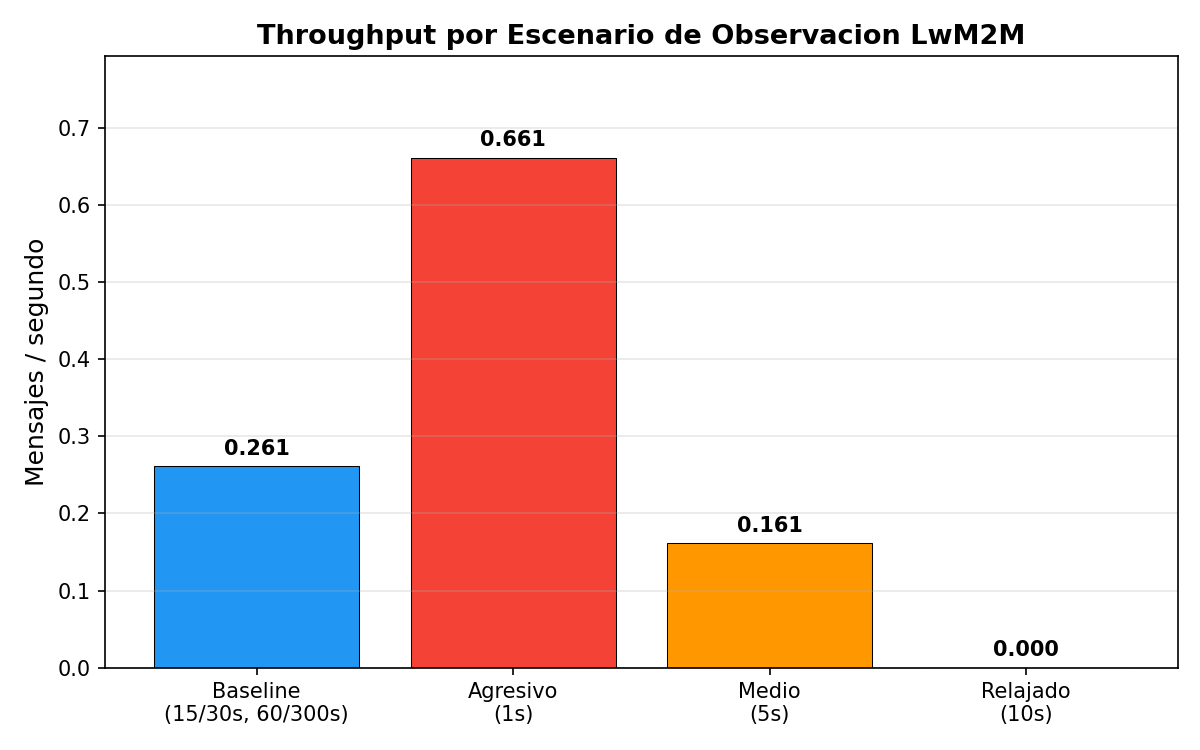
\includegraphics[width=0.68\textwidth]{figures/benchmark_v0151_throughput}
\caption{\emph{Throughput} LwM2M del firmware final v0.15.1 por escenario Observe.}
\label{fig:rpt-v0151-throughput}
\end{figure}

% ============================================================
\section{Detalle por Intervalo Observe}
% ============================================================

La Tabla~\ref{tab:v0151-detail} detalla el comportamiento del firmware final
(v0.15.1) en los 4 escenarios de intervalo Observe.

\begin{table}[htbp]
\centering
\caption{Detalle de rendimiento v0.15.1 por escenario Observe}
\label{tab:v0151-detail}
\begin{tabular}{lcccc}
\toprule
\textbf{Métrica} & \textbf{Baseline} & \textbf{1\,s} & \textbf{5\,s} & \textbf{10\,s} \\
\midrule
Mensajes totales     & 47    & 119   & 29    & 0 \\
Throughput (msgs/s)  & 0,261 & 0,661 & 0,161 & 0,000 \\
Keys reportadas (/16)& 16    & 16    & 16    & 0 \\
Duración captura (s) & 180   & 180   & 180   & 180 \\
\bottomrule
\end{tabular}
\end{table}

\textbf{Observaciones:}
\begin{itemize}
    \item El escenario \textbf{10\,s} genera \textbf{0 mensajes}: el período
    máximo ($p_{max}$) resulta inferior al intervalo de lectura DLMS, por lo
    que ningún valor supera el umbral de notificación.
    \item El escenario \textbf{1\,s} (agresivo) genera 2,5$\times$ más mensajes
    que baseline, confirmando que los umbrales actúan como filtro proporcional.
\end{itemize}

\begin{figure}[htbp]
\centering
\subfigure[Distribución IAT por escenario]{%
    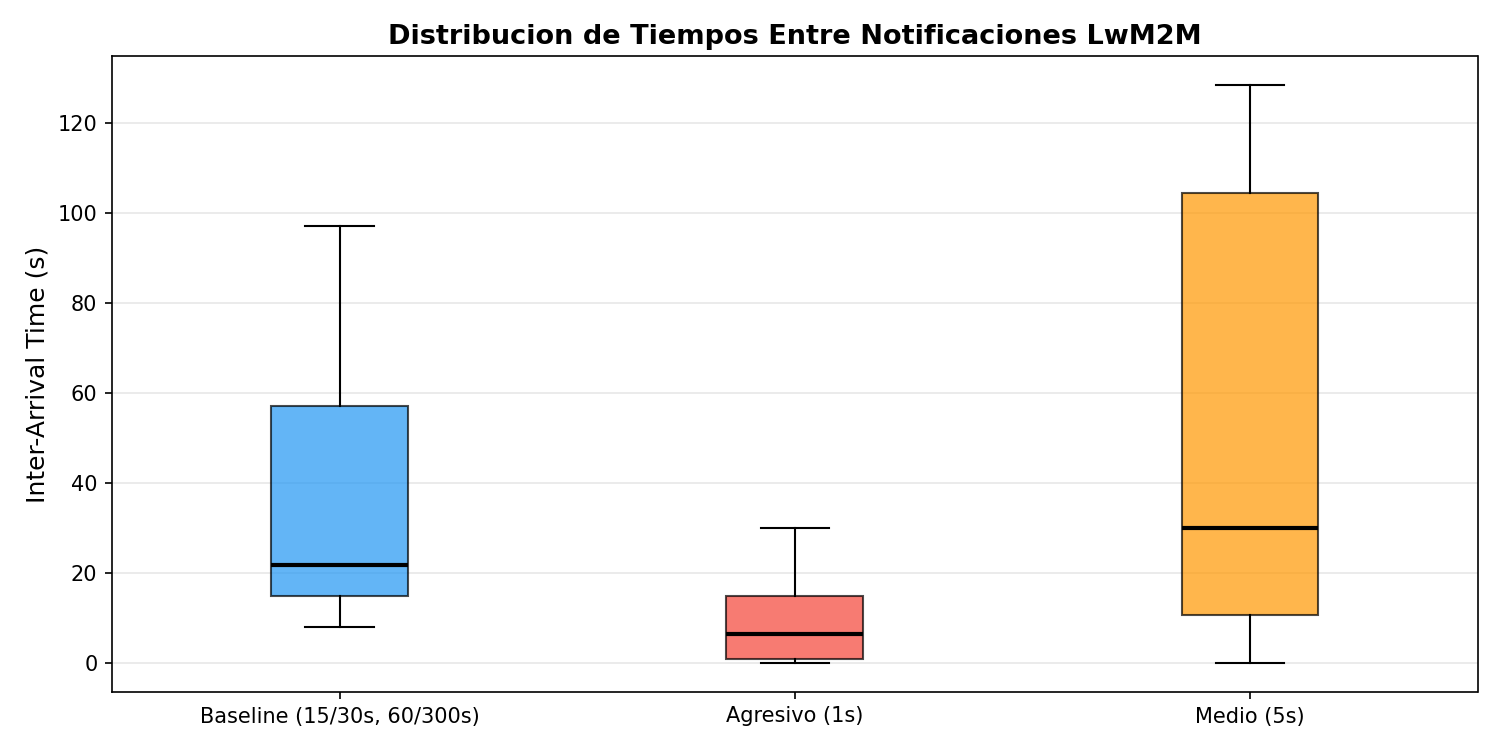
\includegraphics[width=0.48\textwidth]{figures/benchmark_v0151_iat_boxplot}%
    \label{fig:rpt-v0151-iat}}%
\hfill
\subfigure[RSSI y LQI por escenario]{%
    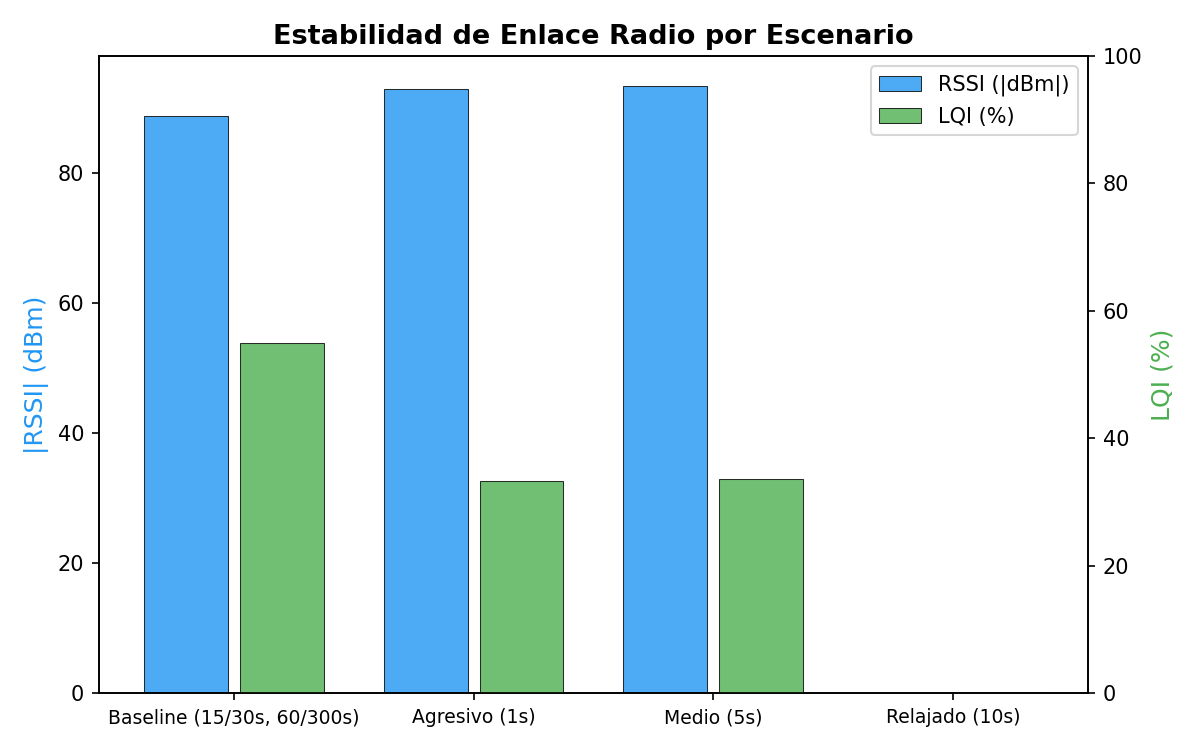
\includegraphics[width=0.48\textwidth]{figures/benchmark_v0151_rssi_lqi}%
    \label{fig:rpt-v0151-rssi}}%
\caption{Caracterización v0.15.1. (a)~IAT del escenario 1\,s promedia 11,46\,s;
baseline 32,33\,s. (b)~RSSI $-$89 a $-$93\,dBm, LQI 33--55\%, operación en zona
marginal ($\sim$15\,m, sin LoS).}
\label{fig:rpt-v0151-detail}
\end{figure}

\begin{figure}[htbp]
\centering
\subfigure[Completitud de keys por escenario]{%
    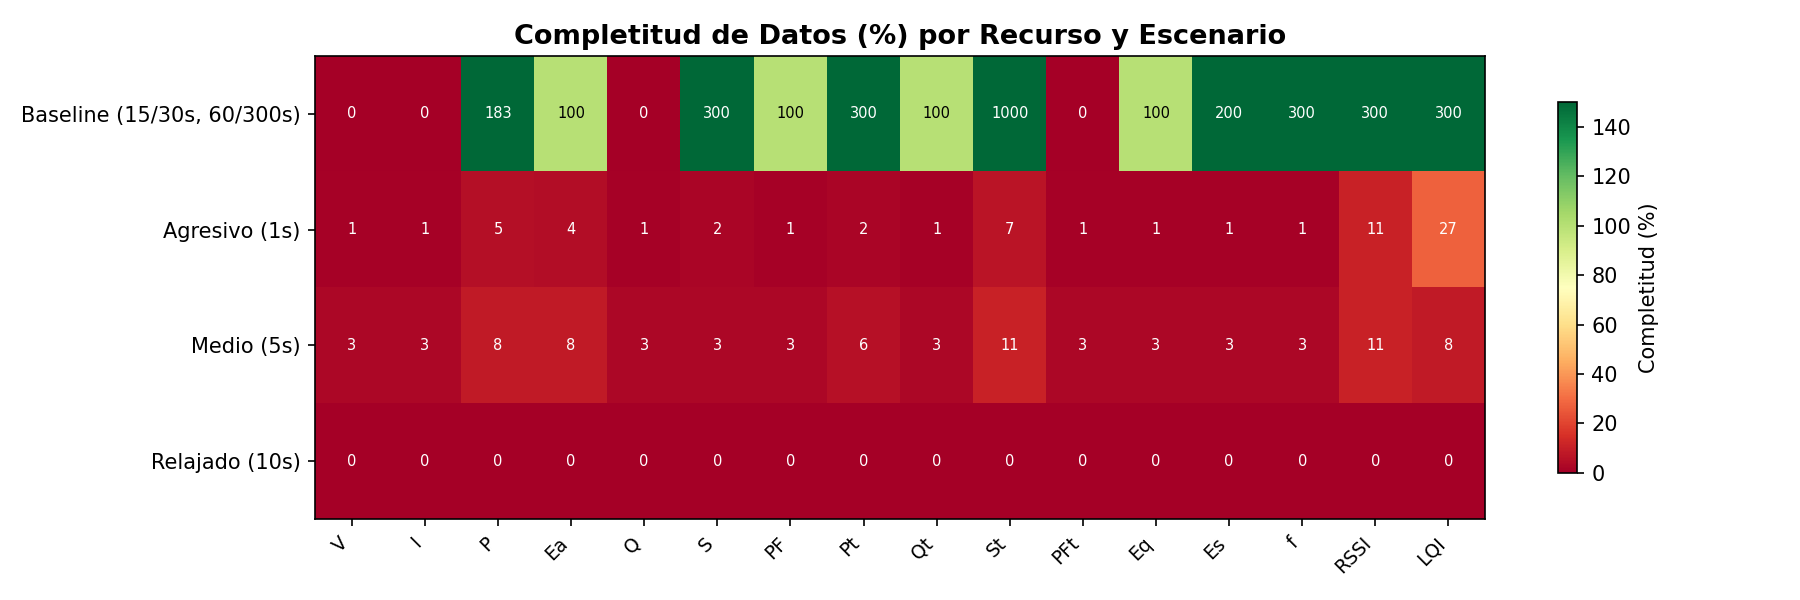
\includegraphics[width=0.48\textwidth]{figures/benchmark_v0151_completeness}%
    \label{fig:rpt-v0151-completeness}}%
\hfill
\subfigure[Overhead CoAP por escenario]{%
    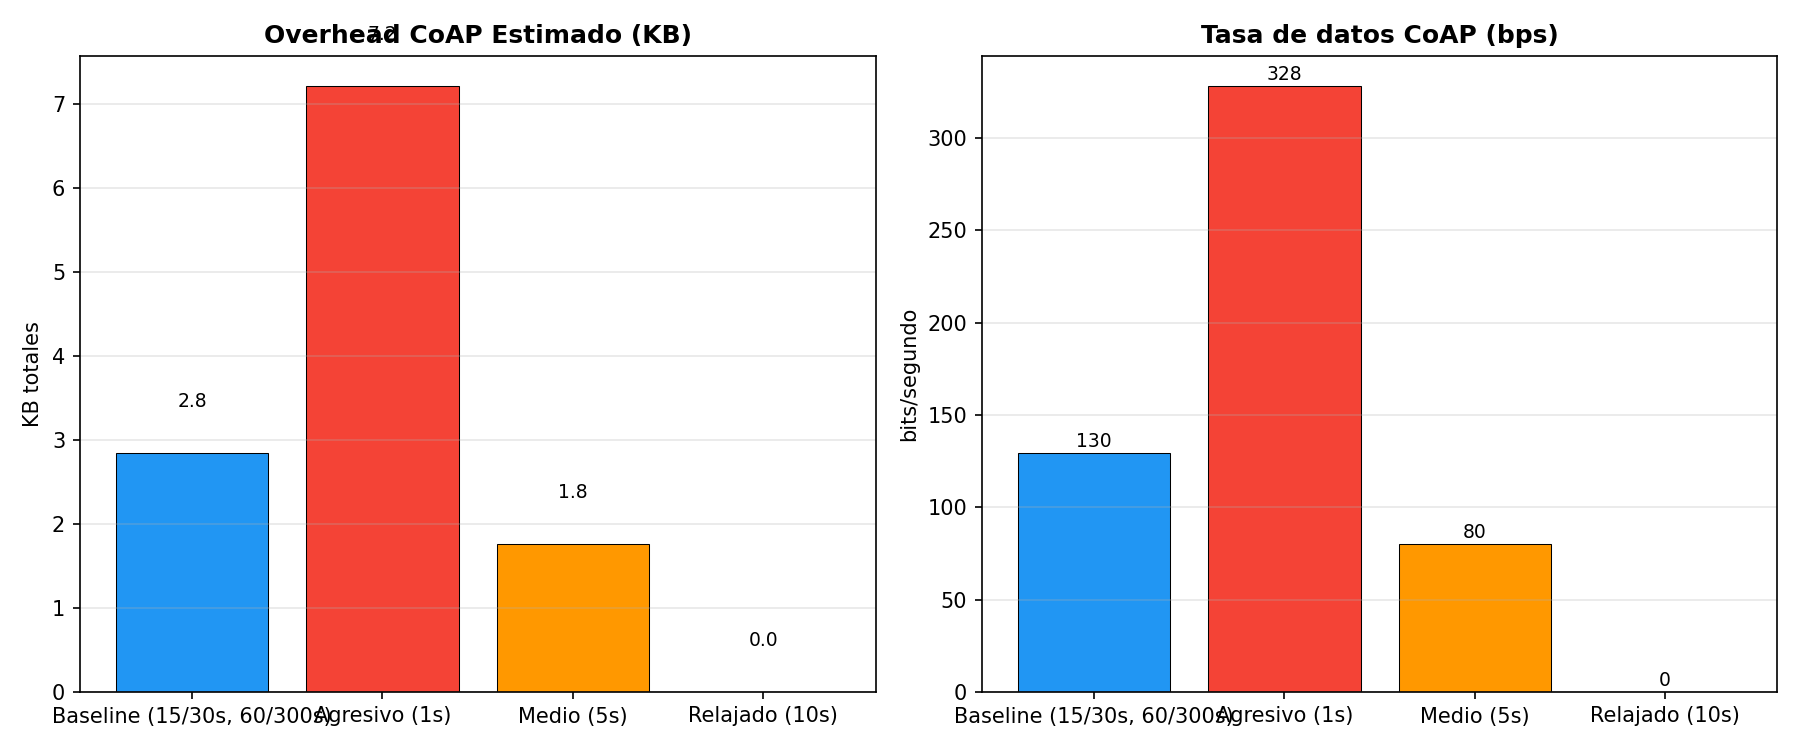
\includegraphics[width=0.48\textwidth]{figures/benchmark_v0151_coap_overhead}%
    \label{fig:rpt-v0151-overhead}}%
\caption{v0.15.1: completitud y overhead. (a)~16/16 keys en baseline, 1\,s y 5\,s;
0/16 en 10\,s. (b)~Overhead CoAP por mensaje en cada escenario.}
\label{fig:rpt-v0151-extra}
\end{figure}

% ============================================================
\section{Análisis Profundo: Utilización del Canal Thread}
% ============================================================

El escenario de 10\,s (600\,s de captura) permite medir la utilización real
del canal IEEE~802.15.4 con un único nodo activo.

\begin{table}[htbp]
\centering
\caption{Análisis profundo del canal Thread (escenario 10\,s, 600\,s de captura)}
\label{tab:deep-analysis}
\begin{tabular}{lr}
\toprule
\textbf{Métrica} & \textbf{Valor medido} \\
\midrule
Tasa de datos radio       & 0,271 kbit/s \\
Utilización del canal      & \textbf{0,22\%} \\
Payload CoAP útil          & 9,69 KB \\
Total bytes radio          & 19,84 KB \\
Eficiencia payload         & 23,6\% \\
Overhead protocolos        & 76,4\% \\
$N_{max}$ estimado (Thread)& \textbf{461 nodos} \\
\bottomrule
\end{tabular}
\end{table}

La estimación de escalabilidad se calcula como:
\begin{equation}
N_{max} = \left\lfloor \frac{BW_{canal} \times U_{objetivo}}{R_{nodo}} \right\rfloor
= \left\lfloor \frac{250 \times 0{,}50}{0{,}271} \right\rfloor = 461 \text{ nodos}
\label{eq:rpt-nmax}
\end{equation}

donde $BW_{canal} = 250$\,kbps (IEEE~802.15.4), $U_{objetivo} = 50\%$ (umbral
práctico de saturación) y $R_{nodo} = 0{,}271$\,kbit/s (medido).

\begin{figure}[htbp]
\centering
\subfigure[Utilización del canal 802.15.4]{%
    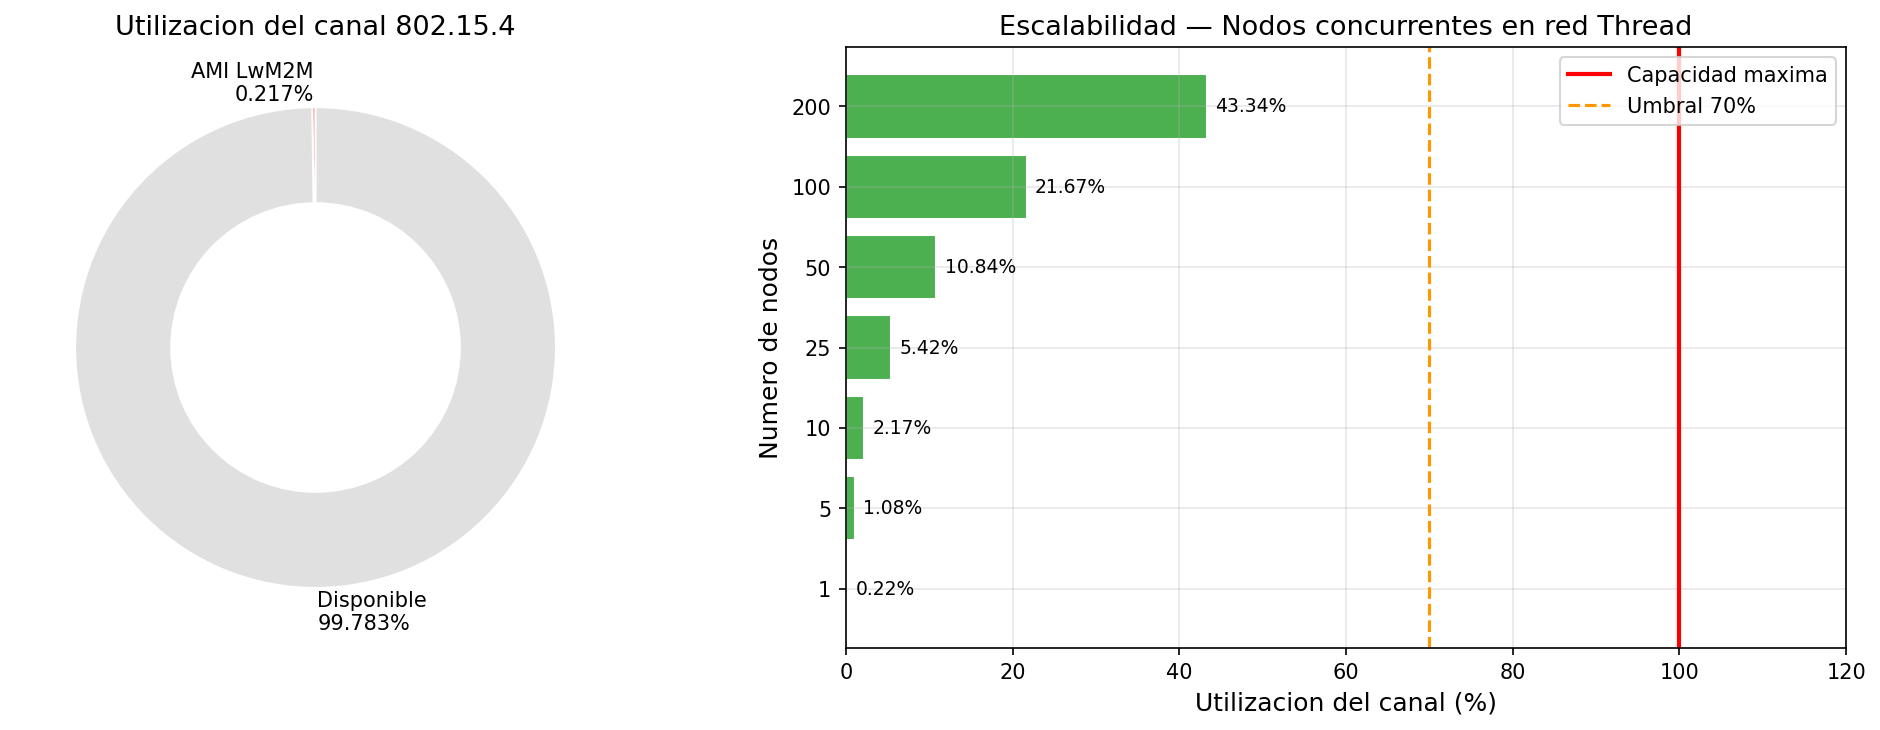
\includegraphics[width=0.48\textwidth]{figures/benchmark_deep_network_util}%
    \label{fig:rpt-deep-network}}%
\hfill
\subfigure[Sobrecarga de protocolos]{%
    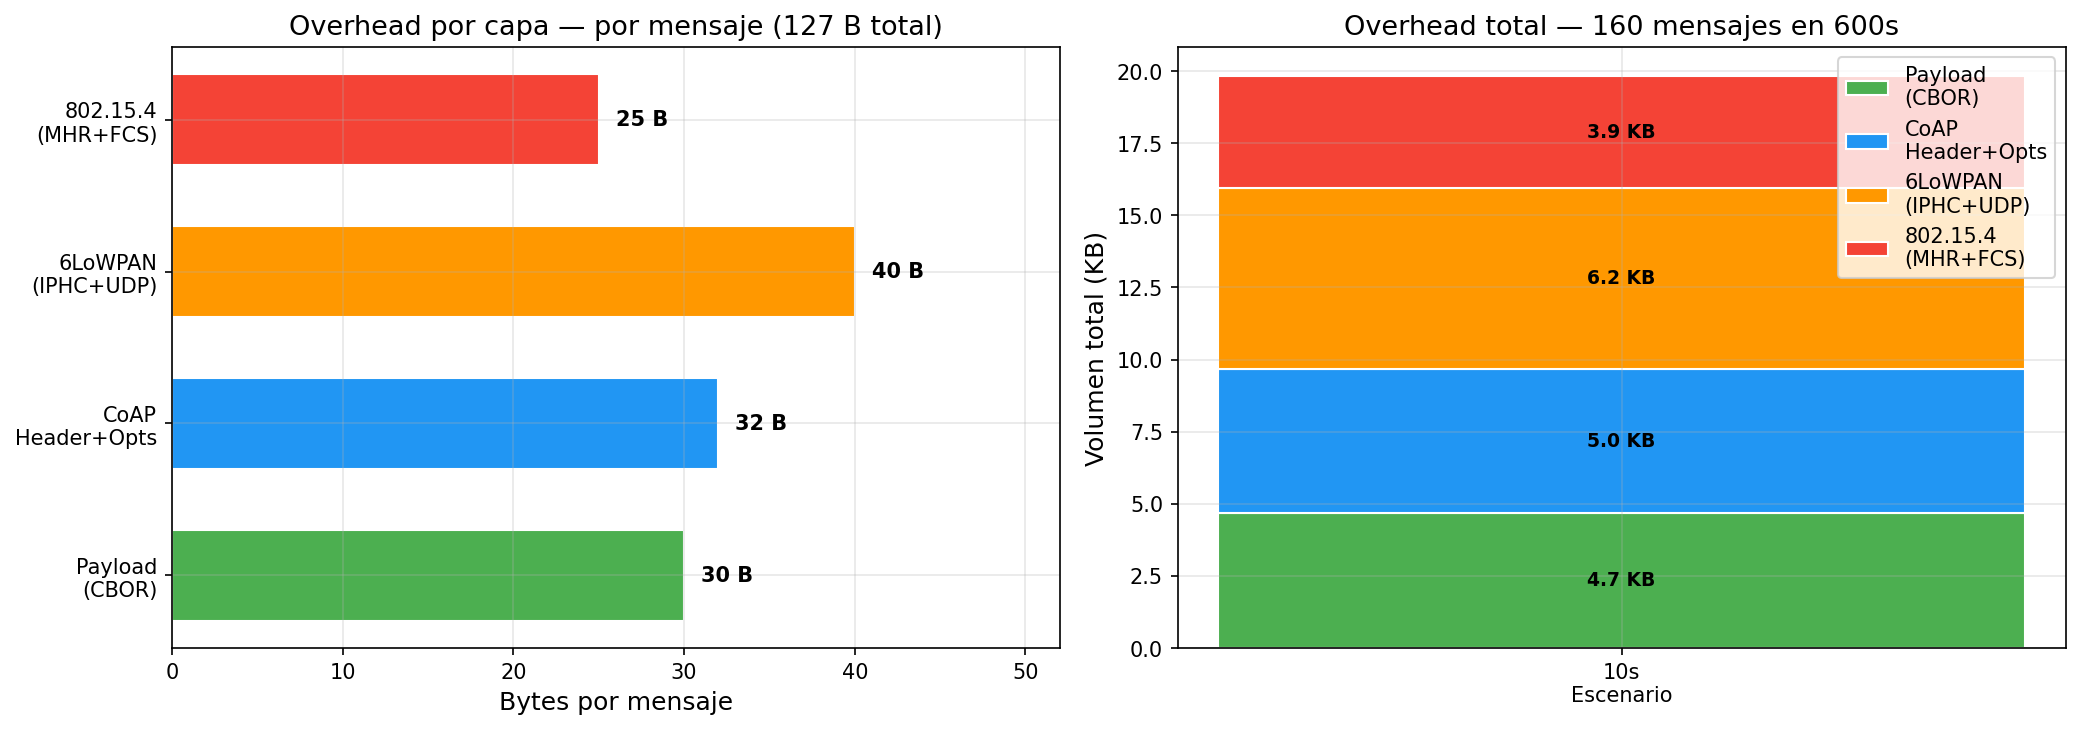
\includegraphics[width=0.48\textwidth]{figures/benchmark_deep_protocol_overhead}%
    \label{fig:rpt-deep-overhead}}%
\caption{Análisis profundo canal Thread. (a)~Utilización 0,22\% de 250\,kbps,
permitiendo hasta 461 nodos. (b)~Eficiencia payload 23,6\% (9,69\,KB CoAP de
19,84\,KB totales en capa radio).}
\label{fig:rpt-deep-analysis}
\end{figure}

\begin{figure}[htbp]
\centering
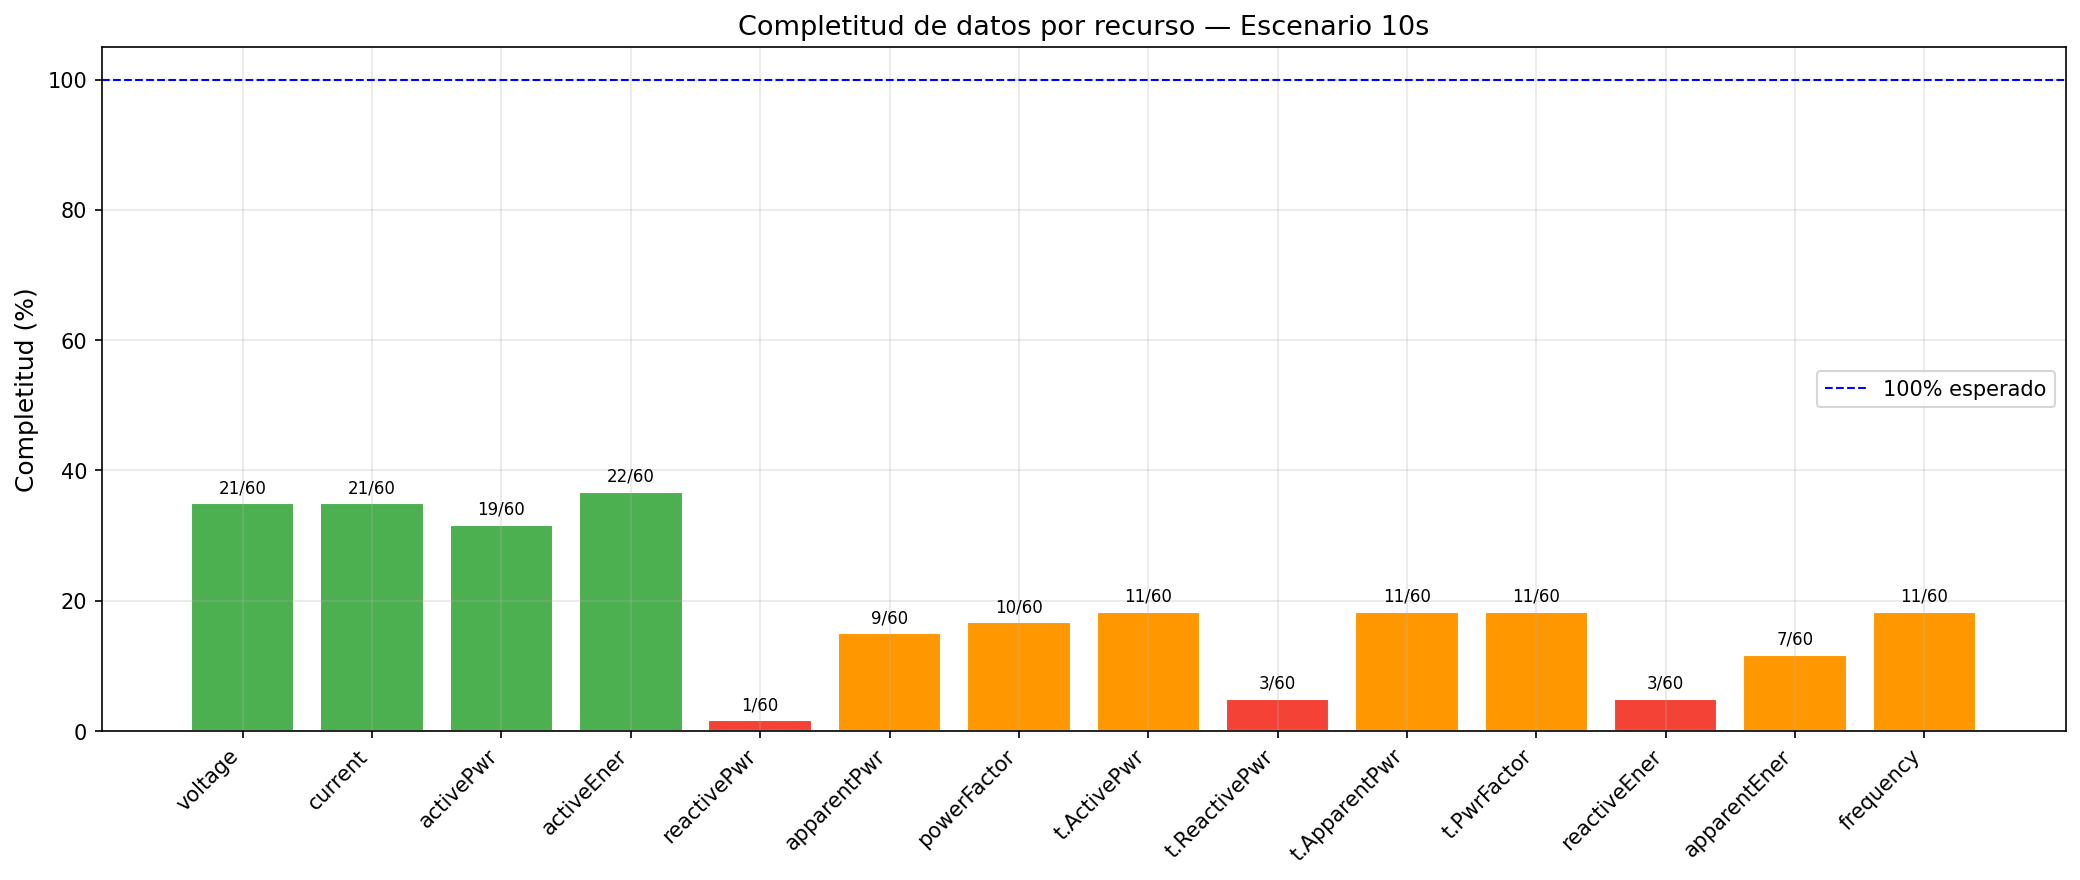
\includegraphics[width=0.65\textwidth]{figures/benchmark_deep_completeness}
\caption{Completitud de keys LwM2M en análisis profundo (10\,s, 600\,s de captura).}
\label{fig:rpt-deep-completeness}
\end{figure}

% ============================================================
\section{Conclusiones del Benchmark}
% ============================================================

\begin{enumerate}
    \item El firmware final v0.15.1 mantiene \textbf{16/16 keys} observables en
    escenarios baseline, 1\,s y 5\,s.

    \item Los umbrales inteligentes (\texttt{THRESH\_CHECK}) reducen señalización
    en escenarios no agresivos, preservando la observabilidad operativa.

    \item El canal Thread opera al \textbf{0,22\%} de su capacidad con un nodo,
    lo que permite estimar hasta \textbf{461 nodos} por red Thread sin superar
    el 50\% de utilización.

    \item La eficiencia del payload (23,6\%) indica un overhead de protocolos
    significativo (CoAP/DTLS/6LoWPAN/802.15.4), lo cual motiva la incorporación
    de CBOR y observación selectiva como trabajo futuro.

    \item El escenario de 10\,s demuestra que \texttt{THRESH\_CHECK} suprime
    completamente la notificación cuando $p_{max}$ es inferior al intervalo
    de lectura DLMS --- comportamiento correcto y deseable para ahorro energético.
\end{enumerate}

\end{document}
